
\newpage
\section{Notes}

Sample file: Links on the class website \url{http://prancer.physics.louisville.edu/classes/308/} \\
Figure \ref{fig:graph1} is an example of  how to do it in \LaTeX \footnote{An example of footnotes}.
\begin{figure}[h]  %t: top, h:exact position
	\begin{center}
	\includegraphics[scale=0.5]{image/good_abstract.png}
	\end{center}
	\caption{The Orion Nebula, M42, recorded with the CDK20N telescope on the night of November 1, 2011.}
	\label{fig:graph1}
\end{figure}

In text $e=mc^2$ and $\frac{1}{2n-1}$.\\

%------------------------------------------
%             tables
%------------------------------------------
\begin{equation}
\frac{x}{y}, \quad
\frac{\delta{f}}{\delta(x)},\quad
\frac{\partial^{2}{f}}{\partial{x}{^2}}
\end{equation}

\cite{Sudsang00_Grasping_In-handManipulation}
\cite{Kalker_1991_RC}
\cite{Yousef_2011_Tactile_Sensing}

    
%------------------------------------------
%             Tikz
%------------------------------------------
\begin{center}
%grid-2D-coordinates

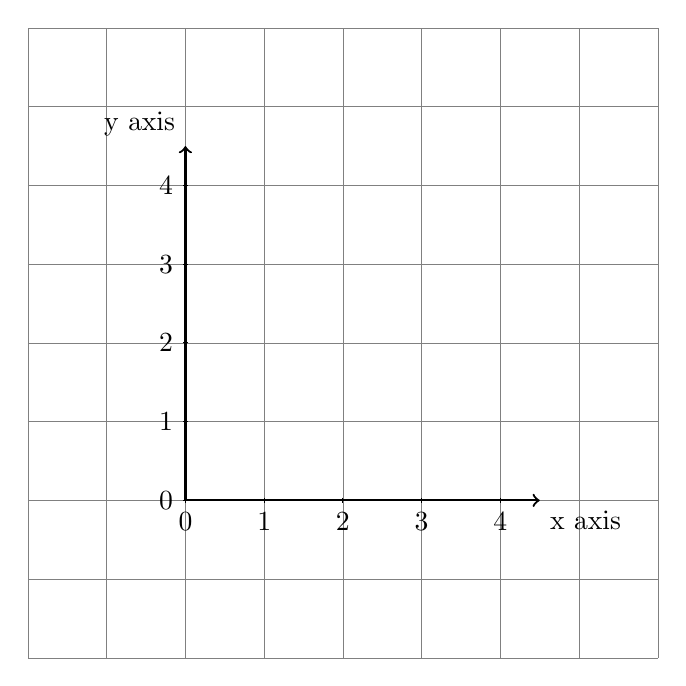
\begin{tikzpicture}
\draw[step=1cm,gray,very thin] (-2,-2) grid (6,6);
\draw[thick,->] (0,0) -- (4.5,0) node[anchor=north west] {x axis};
\draw[thick,->] (0,0) -- (0,4.5) node[anchor=south east] {y axis};

\foreach \x in {0,1,2,3,4}
   \draw (\x cm,1pt) -- (\x cm,-1pt) node[anchor=north] {$\x$};
\foreach \y in {0,1,2,3,4}
    \draw (1pt,\y cm) -- (-1pt,\y cm) node[anchor=east] {$\y$};

\end{tikzpicture}

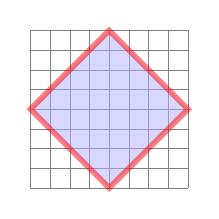
\begin{tikzpicture}
	\draw[step=0.25cm,gray,very thin] (-1,-1) grid (1,1);
	\draw[fill,color=blue!30,draw=red,line width=2pt, opacity=0.5] (1,0) -- (0,1) -- (-1,0) -- (0,-1) -- cycle;
\end{tikzpicture}

\begin{tikzpicture}
	\draw (0,0) grid(5,6);
	\draw (-2,8) rectangle(0,0);
	\draw (0,0) circle (2);
	\draw (5,5) circle (3 and 5);
	\draw (5,8) arc(-90:90:5);
\end{tikzpicture}


\end{center}

%rotation coordinate1
\tdplotsetmaincoords{60}{110}

\begin{tikzpicture}[scale=3,tdplot_main_coords]
\draw[thick,->] (0,0,0) -- (1,0,0) node[anchor=north east]{$x$};
\draw[thick,->] (0,0,0) -- (0,1,0) node[anchor=north west]{$y$};
\draw[thick,->] (0,0,0) -- (0,0,1) node[anchor=south]{$z$};
\coordinate (Shift) at (2,2,2);
\tdplotsetrotatedcoords{-20}{10}{0}
\tdplotsetrotatedcoordsorigin{(Shift)}
\draw[thick,color=blue,tdplot_rotated_coords,->] (0,0,0)
-- (1,0,0) node[anchor=south east]{$x'$};
\draw[thick,color=blue,tdplot_rotated_coords,->] (0,0,0)
-- (0,1,0) node[anchor=west]{$y'$};
\draw[thick,color=blue,tdplot_rotated_coords,->] (0,0,0)
-- (0,0,1) node[anchor=south]{$z'$};
\tdplotsetrotatedthetaplanecoords{30}
\draw[thick,color=blue,tdplot_rotated_coords,->] (0,0,0)
-- (.5,0,0) node[anchor=south east]{$x''$};
\draw[thick,color=blue,tdplot_rotated_coords,->] (0,0,0)
-- (0,.5,0) node[anchor=west]{$y''$};
\draw[thick,color=blue,tdplot_rotated_coords,->] (0,0,0)
-- (0,0,.5) node[anchor=south]{$z''$};
\end{tikzpicture}


\input{coord_rotation2}

\newpage
\begin{center}
\begin{figure}
\subfigure[abc]{
%rotation coordinate1
\tdplotsetmaincoords{60}{110}

\begin{tikzpicture}[scale=3,tdplot_main_coords]
\draw[thick,->] (0,0,0) -- (1,0,0) node[anchor=north east]{$x$};
\draw[thick,->] (0,0,0) -- (0,1,0) node[anchor=north west]{$y$};
\draw[thick,->] (0,0,0) -- (0,0,1) node[anchor=south]{$z$};
\coordinate (Shift) at (2,2,2);
\tdplotsetrotatedcoords{-20}{10}{0}
\tdplotsetrotatedcoordsorigin{(Shift)}
\draw[thick,color=blue,tdplot_rotated_coords,->] (0,0,0)
-- (1,0,0) node[anchor=south east]{$x'$};
\draw[thick,color=blue,tdplot_rotated_coords,->] (0,0,0)
-- (0,1,0) node[anchor=west]{$y'$};
\draw[thick,color=blue,tdplot_rotated_coords,->] (0,0,0)
-- (0,0,1) node[anchor=south]{$z'$};
\tdplotsetrotatedthetaplanecoords{30}
\draw[thick,color=blue,tdplot_rotated_coords,->] (0,0,0)
-- (.5,0,0) node[anchor=south east]{$x''$};
\draw[thick,color=blue,tdplot_rotated_coords,->] (0,0,0)
-- (0,.5,0) node[anchor=west]{$y''$};
\draw[thick,color=blue,tdplot_rotated_coords,->] (0,0,0)
-- (0,0,.5) node[anchor=south]{$z''$};
\end{tikzpicture}


}
\hfill
\subfigure[abc]{
\input{coord_rotation2}
}
\end{figure}
\end{center}

%------------------------------------------
%             Objectives
%------------------------------------------
\subsection*{How to write Objectives}
"Provide a clearly defined statement of the objectives of the research." Sometimes only one objective; sometimes one board AIM, and several objectives.\\
Use active verbs, i.e. propose, create, construct, demonstrate, define, establish, differentiate.
\begin{enumerate}[(i)]
  \item The labels consists of sequential numbers.  
  \begin{itemize}
  	\item The individual entries are indicated with a black dot, a so-called bullet.
  	\item The text in the entries may be of any length.
  \end{itemize}
  \item The numbers starts at 1 with every call to the enumerate environment.
\end{enumerate}
%-------------------------------------------------------
%				Dexterous Motion Planning
%-------------------------------------------------------
\noindent\uline{Dexterous motion planning.} The robot dexterous ma


While Okamura \cite{Okamura_2000_Overview_DM} divided dexterous motion planning into two main categories including the motion planning of the object to acquire a desired configuration and the grasp planning in terms of contact forces optimization.\\

\cite{Trinkle90_Planning_DexManipulation, Trinkle_1991_framework_Planning_DM, Munoz95_Dex.Manipulation_Geo}\\

The article \cite*{Bicchi_2000_Hands_Dexterous} focused on three main categories namely manipulative dexterity, grasp robustness, and human operability.
\begin{enumerate}
    \item{Manipulative dexterity: the capability of the hand to manipulate objects so as to relocate them arbitrarily for the purposes of the tasks.}
    \item{Grasp robustness is the capability of keeping hold of manipulated objects in spite of all possible disturbances (unexpected forces, erroneous estimates of the object characteristics, etc.) while maintaining a "gentle” enough grip not to cause any damage.}
	\item{Human operability: the allowance for an easy and friendly interface with the human operator.}
\end{enumerate}
%------------------------------------------
%             Dr. Lei Research Proposal
%------------------------------------------
\newpage
\subsection{Dr. Lei Research Proposal}
\subparagraph{1-Aim}
\textcolor{red}{To develop a discrete rolling contact theory for tactile fingertips.}\\

\noindent\uline{Lack of discrete contact theory for tactile fingertips.} Tactile fingertips have been increasingly used in robot hands in recent years to enhance their dexterity and adaptability. The geometric differential properties of the discretised fingertip surfaces need to be approximated to be used. In this respect, tools such as the \textbf{moving frame} and \textbf{curvatures in discrete differential geometry} provide a consistent and computationally efficient method to approximate these entities. However, \textcolor{red}{\textbf{these tools have not been applied to in-hand manipulation}.}\\


\noindent\uline{Novelty and Impact.} This project will also employ the \emph{tools} developed in \emph{discrete differential geometry} \textbf{to establish \textcolor{red}{a discrete contact theory} of discrete surfaces}, which will be integrated into the proposed pure geometric framework. This project will eradicate the barriers that have hindered the progress of in-hand manipulation and enable robot hands to be used in advanced manufacturing and ultimately to have dexterity and adaptability comparable to the human hand.\\

\subparagraph{2-Background}
\begin{itemize}
\item Rolling contact in human in-hand manipulation
\item Rolling contact in robot hands
\item Vectorial kinematics of multifingered hands
\item Lie group and Lie algebra in kinematics multifingered hands
\item Contact theory via Cantan’s moving frame method
\item Singularity theory for in-hand manipulation
\item \textbf{Discrete contact theory for tactile fingertips}. In recent years, tactile sensors have been added to fingertips of robot hands to emulate human sensing in grasping and manipulation \cite{Lei-Bagnell12_Tactile_Autonomous, HaoDang11_Tactile_BlindGrasping, Rothling07_Dex.Manipulators_Tactile, Zhang14_Tactile_DynamicGrasping}. These grid-based tactile sensors naturally discretise the surfaces of fingertips into \emph{quadrilateral faces}, where the discrete equivalents of notions and methods in differential geometry, such as \textbf{curvatures and the moving frame method}, can be extended \cite{Bobenko10_Discrete_Curvature, Sullivan08_Curvature_DiscreteSurface}. 

Recent progress in discrete differential geometry introduces tools to \textbf{approximate geometric attributes}, especially \textbf{the moving frames and curvatures}, which are guaranteed \emph{to be appropriate extension from the continuous to the discrete setting} \cite{Meyer03_Discrete_Diff.Geo_2Manifolds, Xu13_Geo.Diff_Discrete, Hameiri03_Darboux_Curvature_Discrete}. However, \textcolor{red}{these new tools have not been applied to in-hand manipulation}.
\end{itemize}



\begin{itemize}
\item [25] H. Dang, J. Weisz, and P. K. Allen, "Blind grasping: Stable robotic grasping using tactile feedback and hand kinematics,"
\item [26] F. Röthling."Platform portable anthropomorphic grasping with the bielefeld 20-dof shadow and 9-dof tum hand," 
\item [27] T. Zhang. "Multifingered robot hand dynamic grasping control based on fingertip three-axis tactile sensor feedback," 
\item [28] A. I. Bobenko."A curvature theory for discrete surfaces based on mesh parallelity,"
\item [29] J. M. Sullivan, "Curvatures of smooth and discrete surfaces," in Discrete differential geometry
\item [30] M. Meyer,"Discrete differential-geometry operators for triangulated 2-manifolds," 
\item [31] G. Xu, "Consistent approximations of several geometric differential operators and their convergence,"
\item [32] E. Hameiri. "Estimating the principal curvatures and the Darboux frame from real 3-D range data,"
\end{itemize}

\subparagraph*{3-Significance} \mbox{}\\

\uline{\textcolor{red}{A new discrete rolling contact theory.}} The moving frame method and curvature theory in differential geometry have their counterparts in discrete differential geometry. \textcolor{blue}{An ever increasing number of robot fingertips are equipped with tactile sensors, and these grid-based sensors naturally mesh the fingertips into discrete surfaces} \cite{Lei14_Teleoperation_ThumbRobotHand,  Bagnell12_IntegratedSystem_AutonomousRoboticsManipulation}.
As I pioneered applying \textcolor{blue}{the curvature theory in differential geometry to in-hand manipulation} \cite{Lei09_coordinate-free_instantaneous_kinematics, Lei10_Darboux-Frame, Lei10_Geometric.Kinematics_PointContact, Lei15_PolynomialFormulation_InverseKinematics, Lei15_sliding.rolling.loci_kinematics, Lei09_Kinematic.Geometry_Circular.Surfaces}, I will initiate applying \textcolor{red}{the discrete} \textcolor{blue}{curvature theory} to in-hand manipulation. I will exploit the rich toolset developed in the communities of discrete differential geometry and computer graphics. I will develop a new discrete contact theory
and integrate it into the proposed geometric framework.

\newpage

\cite{Belta_2005_Discrete_MP} (Discrete abstractions for robot motion planning and control in polygonal environments)
\subparagraph{4-Research Design and Method}
\subparagraph*{Overview} Further, I will develop a new discrete contact theory by extending my pioneering work and applying the recent progress in discrete differential geometry.\\

\textbf{Aim 2}: \textbf{To develop a discrete contact theory.}\\

\uline{\textbf{Rationale}}. The grid-based tactile sensors naturally discretise the fingertip surfaces into quadrilateral faces, which can be converted into triangle meshes that have been extensively used in Computer Graphics \cite{Martin04_Quadrilateral_Discrete}. Contact theory requires an approximation of the first and second order properties, such as curvatures and principle directions \cite{Lei10_Darboux-Frame, Montana88_Kinematics_Contact_Grasp}. The current patch-based contact theory needs analytical evaluation, which often introduces overshooting or unexpected surface behaviour. 

On the other hand, moving frame and curvatures can be consistently derived by the rich tool set developed in discrete differential geometry, and these appropriations are guaranteed to be an extension from the continuous to the discrete setting \cite{Meyer03_Discrete_Diff.Geo_2Manifolds}.\\

\uline{\textbf{Theoretical approach}.} I propose to apply \emph{the tool set} developed in \textbf{discrete differential geometry to establish a discrete contact theory}. My contact theory for smooth surfaces is formulated in terms of the moving frame, normal curvature, geodesic curvature, and geodesic torsion [\cite{Lei09_coordinate-free_instantaneous_kinematics, Lei10_Darboux-Frame, Lei15_PolynomialFormulation_InverseKinematics, Lei15_sliding.rolling.loci_kinematics, Lei10_PhDThesis}. \emph{Each of these geometric entities has its counterpart in discrete differential geometry}, as in Fig. 5 (Lei's PhD thesis \cite{Lei10_PhDThesis}). When I was deriving the contact theory, the velocity constraint was embedded in the arc length, \textcolor{red}{eliminating the need of nonlinear differential equations} and \textcolor{blue}{facilitating grid-based path planning}, as in Fig. 6 (in \cite{Lei09_coordinate-free_instantaneous_kinematics}). I \emph{will apply the same approach} in the \emph{discrete case} \textbf{to establish a discrete contact theory} that is coordinate-independent and does not involve difference terms.\\


\uline{\textbf{Empirical validation}.} The BarrettHand is equipped with tactile sensors capable of providing 96 cells of tactile-array data spread across all three fingers and the palm. The density of cells becomes higher towards the very tips of the fingers where finer spatial resolution is desirable \cite{Martin04_Quadrilateral_Discrete}. The embedded signal processing of raw data from the tactile sensors can determine point of contact, and this will facilitate validation of the proposed discrete contact theory.

\subparagraph{Reference}
\begin{itemize}
\item 1 From Dr.LeiCui research : \cite{Lei10_Darboux-Frame, Lei10_Geometric.Kinematics_PointContact, Lei11_Posture.Workspace_Multifinger, Lei12_Polynomial_Inverse.Kinematics, Lei12_ReciprocityBased_SVD_Inverse.Kinematics, Lei15_sliding.rolling.loci_kinematics, Lei15_PolynomialFormulation_InverseKinematics, Lei18_Rolling.Contact_Kinematics_Multifinger, Lei17_In-Hand_Forward.Inverse.Kinematics, Lei07_Euclidean_Invariants, Lei09_Kinematic.Geometry_Circular.Surfaces, Lei09_Orientation-Workspace_Metahand, Lei09_coordinate-free_instantaneous_kinematics}
\item 2 Text book about dynamic-discrete \cite{Book_Rosenberg77_DynamicsDiscrete}
\end{itemize}


%==============================================================
\subsection{Markov Decision Process}
\noindent\uline{Introduction.} 
Markov Decision Process (MDP) is an extension of a Markov chain which is a stochastic model in discrete time. MDP represents a mathematical framework to model decision making process that has been studied in early \cite{Howard60_DP_MDP, Miller68_MDP}. For the record, many applied study may have an implicit underlying the MDP framework to determine the expected cost of raw material that the stock can purchase or shortage \cite{White85_ApplicationMDP}, to control the pest or protect natural resources \cite{White93_ApplicationMDP}. In the robotic field, the MDP has been successfully applied for path planning problems such as combination with a quadtree decomposition of the environment to compute the motion plan \cite{Burlet04_MP_MDP} or association with ideas of deterministic search and dynamic programming techniques to reduce the processing cost and improve performance path planning algorithm \cite{Ferguson04_MDP_Pathplanning}. Another promising technique for autonomous trajectory planning is based on the MDP with clothoid tentacles \cite{Muhager16_MDP_Clothes}. The study used stochastic transitions \cite{Puterman14_Book_MDP_DiscreteDP} that can reduce the presence of distant obstacles in an occupancy grid.\\


%==============================================================
\noindent\uline{The agent-environment interface.} 
As shown in Figure \ref{fig:MDP1}, there are two main objects in the MDP including an agent and the environment that they interact together at each of a sequence of discrete time steps, $t=0,1,2,3,...$. The process in some states $S_t$ at each time step $t$ is described that the decision maker chooses any action $A_t$ in the state and the agent will receive the reward $R_t$ from the environment. In \cite{SuttonBarto18_RLbook}, the general rule of agent-environment boundary is not the same as the physical boundary of a robot's or animal's body. In some cases, the agent may know everything in the environment, just as the rewards which are computed from the agent's action function or the state received. However, in another case of solving puzzle like Rubik's cube, the agent knows all the environment such as colors, faces and dimensions but hard to solve its work.
\begin{figure}[h]
	\begin{center}
	\includegraphics[width=0.5\textwidth]{image/SuttonBartoI_RL.png}
	%\includegraphics[scale=0.5]{image/MDP.png}
	\end{center}
	\caption{The interaction of agent and environment \cite{SuttonBarto18_RLbook}.}
	\label{fig:MDP1}
\end{figure}


%==============================================================
\noindent MDP is a tuple $<S,A,T,r,\gamma>$ where $S$ is a set of observations when the agent observes a state from the environment; $S$ is a set of actions that the agent can execute from the task to interact with the environment; $T$ is transition probability matrix in which of making the action $a \in A$ from the current state $s \in S$ to the next state $s'$ ($T(s'|s,a)=\mathbb{P}[S_t=s, A_t=a]$); $r$ is the reward model that the agent can receive in the state $s$ when executing an action $a$ ($r(s,a)=\mathbb{E}[R_{t+1}|S_t=s, A_t=a]$), and $\gamma$ is the discount factor where $0<\gamma<1$ that relatives between immediate and future rewards. In path planning problems, the MDP method is applied for finding the path in terms of optimizing the expected sum of discounted rewards and the Bellman equation \cite{Bellman57_MDP} can be promoted in the study.\\ 

%==============================================================
%\noindent\uline{Reinforcement learning.} RL is one part of machine learning which does not require the environment model or the dynamic system as well. \\


%==============================================================
\noindent\uline{Bellman equation.} Before discussing the Bellman equation, there are some of principal components of the Reinforcement Learning framework including Reward and Return, Policies, and Value functions which are briefly introduced as following. \\
\noindent In reinforcement learning, there are two types of value function used to optimize the policy including the state value function $
V^{\pi}(s)=\mathbb{E}_{\pi}[R_t|s_t=s]
$ and the action value function $
Q^{\pi}(s,a)=\mathbb{E}_{\pi}[s_t=s,a_t=a]
$. They are the expected returns generated from the state and action under the policy $\pi$.
The value function changes dependently on the policy for the same environment due to that fact that the value of the state changes dependently and expected rewards will be received. The action value function represents the value of taking an action in some state $s$.\\

\noindent If we call $\mathcal{P}$ is the transition probability from starting state $s$, taking action $a$, then ending up in state $s'$, we have 
$
\mathcal{P}^a_{ss'}=pr(s_{t+1}=s'|s_t=s,a_t=a)
$. 
In addition, $\mathcal{R}^a_{ss'}$ is called the expected reward received from starting state $s$, taking action $a$, and moving into state $s'$, we have 
$
\mathcal{R}^a_{ss'}=\mathbb{E}[r_{t+1}|s_t=s,s_{t+1}=s',a_t=a]
$

\noindent Finally, the Bellman equation \cite{Bellman57_MDP} can be derived for the on-policy state value function with the results is as follows:
\begin{equation}
V^{\pi}(s) = \sum_{a}\pi(s,a)\sum_{s'}\mathcal{P}^a_{ss'}[\mathcal{R}^a_{ss'}+\gamma{V}^{\pi}(s')]
\end{equation}
and for the on-policy action value function as:
\begin{equation}
Q^{\pi}(s,a) = \sum_{s'}\mathcal{P}^a_{ss'}[\mathcal{R}^a_{ss'}+\gamma\sum_{a'}\pi(s',a'){Q}^{\pi}(s',a')]
\end{equation}
for all $s\in{S}, a\in{A(s)}$.

\noindent It is noticed that the Bellman equation can represent the values of states as values of other states like easily calculating the value of state $s_t$ when knowing the value of state $s_{t+1}$. However, to apply for the stochastic shortest path problems by using the Bellman equation, there are techniques such as  value iteration, policy iteration, and linear programming should be taken into consideration to solve the Bellman equation. \\

%==============================================================
\noindent\uline{Value iteration.} This is one of the method to find an optimal policy is to determine the optimal value function. The method in detail to converge to the correct $V^*$ values that can be performed by an iterative algorithm \cite{Bellman57_DynamicProgramming, Bertsekas87_DynamicProgramming}. The Bellman equation for the optimal value function is as follows:
\begin{equation}
Q^{*}(s,a) 
= \mathbb{E}[R_{t+1} + \gamma \max_{a'}Q^{*}(S_{t+1},a')|S_{t}=s, A_{t}=a] 
= \sum_{s',r}p(s',r|s,a)[r+\gamma \max_{a'}Q^{*}(s',a')] 
\end{equation}
The algorithm will stop when the value function changes in a small amount of one update of each state (sweep). The combination of one sweep of policy evaluation and one sweep of policy improvement in the value iteration algorithm can make the convergence faster. It is also noted that the value iteration can be obtained when the step of updating the Bellman optimality equation happens and the updated value has to be required maximum over all actions. \\

%==============================================================
\noindent\uline{Policy iteration.} Policy iteration algorithm can be defined as another way of determining an optimal policy in a finite number iteration. The iteration starts with the value function $V(s)$ of the previous policy $\pi$ in each policy iteration as $\pi_0\xrightarrow{E}v_{\pi_0}\xrightarrow{I}\pi_1\xrightarrow{E}v_{\pi_1}\xrightarrow{I}\pi_2\xrightarrow{E} ... {\pi_*}\xrightarrow{E}v_*$, where $\xrightarrow{E}$ denotes a policy evaluation and $\xrightarrow{I}$ indicates a policy improvement. The Bellman equation for the optimal value function as the policy iteration is:
\begin{equation}
V^{*}(s) 
= \max_{a} \mathbb{E}[R_{t+1} + \gamma V^{*}(S_{t+1})|S_{t}=s, A_{t}=a] = \max_{a} \sum_{s',r}p(s',r|s,a)[r+\gamma V^{*}(s')]
\end{equation}
The policy iteration algorithm may converge only few iterations that will be gained the expected infinite discounted reward by executing the policy \cite{SuttonBarto18_RLbook}: 
\begin{equation}
\pi'(s)=argmax_{a}(R(s,a)+\gamma \sum_{s'\in S} p(s',r|s,a)V^{\pi}(s'))
\end{equation}

%==============================================================
\noindent\uline{Linear programming.} Linear programming methods can be used to solve the Bellman equation and they are better than dynamic programming in some cases as less number of states and a potential method in the curse of dimensionality.
The significant application of the linear programming based path planning algorithm is to derive optimal paths for robotics in various kinds of environment \cite{Chasparis05_PP_LinearProgramming}. The article proposed a linear formulation for resource allocation of the path planning issue. Integrating linear programming to a receding horizon implementation for multi-vehicle path planning is introduced as a model simplification. To describe the feasible path planning, the paper also used stochastic models which can propose the current position and predict the future trajectories. Another implementation of linear programming from \cite{Yang12_PP_LinearProgramming} for the path planning problems has been focus on obstacle avoidance. The most advantage of this improvement is to reduce the computation time cost in the real time computation for the path planning process.